\documentclass[11pt,a4paper]{article}

\usepackage[margin=1in, paperwidth=8.3in, paperheight=11.7in]{geometry}
\usepackage{amsfonts}
\usepackage{amsmath}
\usepackage{amssymb} 
\usepackage{enumerate}
\usepackage{enumitem}
\usepackage{fancyhdr}
\usepackage{graphicx}
\usepackage{hyperref}

\begin{document}

\pagestyle{fancy}
\setlength\parindent{0pt}
\allowdisplaybreaks

\renewcommand{\headrulewidth}{0pt}

% Cover page title
\title{Machine Learning - Notes}
\author{Dom Hutchinson}
\date{\today}
\maketitle

% Header
\fancyhead[L]{Dom Hutchinson}
\fancyhead[C]{Machine Learning - Notes}
\fancyhead[R]{\today}

% Counters
\newcounter{definition}[section]
\newcounter{example}[section]
\newcounter{notation}[section]
\newcounter{remark}[section]
\newcounter{theorem}[section]
\newcounter{proof}[section]
\newcounter{proposition}[section]

% commands
\newcommand{\dotprod}[0]{\boldsymbol{\cdot}}
\newcommand{\cosech}[0]{\mathrm{cosech}\ }
\newcommand{\cosec}[0]{\mathrm{cosec}\ }
\newcommand{\sech}[0]{\mathrm{sech}\ }
\newcommand{\blocks}[0]{\mathbb{B}}
\newcommand{\nats}[0]{\mathbb{N}}
\newcommand{\reals}[0]{\mathbb{R}}
\newcommand{\eg}[0]{\textit{e.g.} }
\newcommand{\ie}[0]{\textit{i.e.} }
\newcommand{\integers}[0]{\mathbb{Z}}
\newcommand{\nb}[0]{\textit{N.B.} }
\newcommand{\prob}[0]{\mathbb{P}}
\newcommand{\expect}[0]{\mathbb{E}}
\newcommand{\var}[0]{\mathrm{var}}
\newcommand{\cov}[0]{\mathrm{cov}}
\newcommand{\argmax}[0]{\mathrm{argmax}}
\newcommand{\argmin}[0]{\mathrm{argmin}}

\newcommand{\x}[0]{\textbf{x}}
\newcommand{\X}[0]{\textbf{X}}
\newcommand{\mub}[0]{\pmb{\mu}}

\newcommand{\definition}[1]{\stepcounter{definition} \textbf{Definition \arabic{section}.\arabic{definition}\ - }\textit{#1}\\}
\newcommand{\definitionn}[1]{\stepcounter{definition} \textbf{Definition \arabic{section}.\arabic{definition}\ - }\textit{#1}}
\newcommand{\proof}[1]{\stepcounter{proof} \textbf{Proof \arabic{section}.\arabic{proof}\ - }\textit{#1}\\}
\newcommand{\prooff}[1]{\stepcounter{proof} \textbf{Proof \arabic{section}.\arabic{proof}\ - }\textit{#1}}
\newcommand{\example}[1]{\stepcounter{example} \textbf{Example \arabic{section}.\arabic{example}\ - }\textit{#1}\\}
\newcommand{\examplee}[1]{\stepcounter{example} \textbf{Example \arabic{section}.\arabic{example}\ - }\textit{#1}}
\newcommand{\notation}[1]{\stepcounter{notation} \textbf{Notation \arabic{section}.\arabic{notation}\ - }\textit{#1}\\}
\newcommand{\notationn}[1]{\stepcounter{notation} \textbf{Notation \arabic{section}.\arabic{notation}\ - }\textit{#1}}
\newcommand{\proposition}[1]{\stepcounter{proposition} \textbf{Proposition \arabic{section}.\arabic{proposition}\ - }\textit{#1}\\}
\newcommand{\propositionn}[1]{\stepcounter{proposition} \textbf{Proposition \arabic{section}.\arabic{proposition}\ - }\textit{#1}}
\newcommand{\remark}[1]{\stepcounter{remark} \textbf{Remark \arabic{section}.\arabic{remark}\ - }\textit{#1}\\}
\newcommand{\remarkk}[1]{\stepcounter{remark} \textbf{Remark \arabic{section}.\arabic{remark}\ - }\textit{#1}}
\newcommand{\theorem}[1]{\stepcounter{theorem} \textbf{Theorem \arabic{section}.\arabic{theorem}\ - }\textit{#1}\\}
\newcommand{\theoremm}[1]{\stepcounter{theorem} \textbf{Theorem \arabic{section}.\arabic{theorem}\ - }\textit{#1}}

% Table of contents
\tableofcontents
\section*{General}
Lecturer - \href{carlhenrik.ek@bristol.ac.uk}{Carl Henrik Ek}\\
Course Website - \url{http://carlhenrik.com/COMS30007/}\\
Course Repo - \url{https://github.com/carlhenrikek/COMS30007}\\
Course Subreddit - \url{https://www.reddit.com/r/coms30007/}

% Start of content
\newpage

\section{Introduction}

\subsection{Motivation}

\definition{Deductive Reasoning}
A method of reasoning in which the premieses are viewed as supplying \underline{all} the evidence for the truth of the conclusion.\\

\definition{Inductive Reasoning}
A method of reasoning in which the premieses are viewed as supplying \underline{some} evidence for the truth of the conclusion, rather than all the evidence. This allows for the conclusion of the \textit{Inductive Reasoning} to be false.\\

\remark{Free-Lunch Theorem}
There are infinite number of hypotheses that perfectly explain the data. Adding a data point removes an infinite number of possibilities, but still leaves infinite possibilities.\\

\remark{The Task of Machine Learning}
When proposing to use machine learning on a task, one should consider the following questions:
\begin{enumerate}[label=\roman*)]
	\item How can we formulate beliefes ad assumptions mathematically?
	\item How can we connect our assumptions with data?
	\item How can we update our beliefs?
\end{enumerate}

\remark{Useful Models are not always True}
Our goal is to understand realisations of a system. If we can then we can equate our model to the system. It is important to note thtat our model does not need to be perfectly true to be useful.

\subsection{Probability Theory}

\definition{Stochastic/Random Variable}
A variable whose value depends on outcomes of random phenomona.\\
\eg $x\sim\mathcal{N}(0,1)$.\\

\definition{Probability Measure,$\prob$}
A function with signature $\prob:\mathcal{F}\to[0,1]$, where $\mathcal{F}$ is a sample space of rv $X$, and fulfils $\int_{-\infty}^{\infty}\prob(x)dx=1$.\\

\definition{Joint Probability Distribution}
A \textit{Probability Measure} for multiple variables, $\prob:X\times Y\to[0,1]$.\\
Let $n_{ij}$ be the number of outcomes where $X=x_i$ and $Y=y_j$ then
$$\prob(X=x_i,Y=y_j)=\frac{n_{ij}}{\sum_{i,j}n_{ij}}$$

\definition{Marginal Probability Distribution}
A \textit{Probability Measure} for one variable when the sample space is over multiple variables.\\
Let $n_{ij}$ be the number of outcomes where $X=x_i$ and $Y=y_j$ then
$$\prob(X=x_i)=\frac{\sum_jn_{ij}}{\sum_{i,j}n_{ij}}$$

\definition{Conditional Probability Distribution}
A \textit{Probability Measure} for a variable, given another variable has a defined value.
Let $n_{ij}$ be the number of outcomes where $X=x_i$ and $Y=y_j$ then
$$\prob(Y=y_j|X=x_i)=\frac{n_{ij}}{\sum_{j}n_{ij}}$$

\example{Joint, Marginal \& Conditional Probability}
The below image shows two marginals distributions in the bottom-left, $X$, \& top-right, $Y$, their joint distribution in the top-left and a conditional in the bottom right $\prob(Y|X=1)$.\\
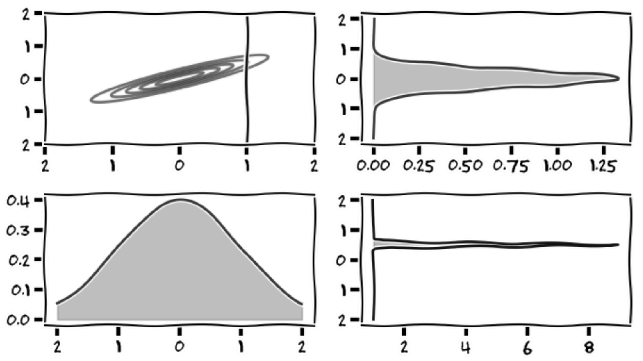
\includegraphics[scale=2]{img/probExamples.png}

\theorem{Product Rule}
For random variables $X$ \& $Y$
$$\prob(X=x,Y=Y)=\prob(Y=y|X=x)\prob(X=x)$$

\theorem{Sum Rule}
For random variables $X$ \& $Y$
$$\prob(X=x)=\sum_j\prob(X=x,Y=y_j)$$

\theorem{Baye's Theorem}
For random variables $X$ \& $Y$
$$\prob(X=x|Y=y)=\frac{\prob(Y=y|X=x)\prob(X=x)}{\prob(Y=y)}$$

\definition{Elements of Bayes' Theorem}
The elements of \textit{Bayes' Theory} can be broken down to explain parts of the model.
$$\underbrace{\prob(\theta|Y)}_{\text{Posterior}}=\frac{\overbrace{\prob(Y|\theta)}^{\text{Likelihood}}\overbrace{\prob(\theta)}^{\text{Prior}}}{\underbrace{\prob(Y)}_{\text{Evidence}}}$$
\begin{tabular}{l|l}
Posterior&Which parameters of the model do I belive produce distributions have generated the data $Y$\\
Likelihood&How likley is the data to come from the model specifely indexed by $\theta$\\
Prior&What distribution do I think parameter $\theta$ has\\
Evidence&How likely do I think data $Y$ is for all models.
\end{tabular}
\nb The \textit{Evidence} normalises this function.\\

\definition{Expectaction Value, $\expect$}
The mean value a random variable will produce from a large number of samples.\\
\begin{tabular}{l|l}
Continuous&Discrete\\\hline
$\expect(X)=\int_{-\infty}^{\infty} x\prob(X)dx$&$\expect(X)=\sum_{-\infty}^{\infty} x\prob(X)dx$\\
$\expect(f(X))=\int_{-\infty}^{\infty} f(x)\prob(X)dx$&$\expect(f(X))=\sum_{-\infty}^{\infty} f(x)\prob(X)dx$
\end{tabular}\\

\definition{Variance}
Describes the amount of spread in the values a single random variable will produce.
$$\var(X)=\expect\left(x-\expect(x))^2\right)=\expect(X^2)-\bigg(\expect(X)\bigg)^2$$

\definition{Covariance}
Describes the joint variability between two random variables.
$$\cov(X,Y)=\expect\bigg(\big(X-\expect(X)\big)\big(Y-\expect(Y)\big)\bigg)$$

\definition{Marginalisation}
The process of summing out the probability of one random variable using its joing probability with another rando variable.
\[\begin{array}{rrcl}
\mathrm{Continuous}&\prob(X=x)&=&\int(X=x,Y=y)dy\\
\mathrm{Discrete}&\prob(X=x)&=&\sum_i\prob(X=x,Y=y_i)
\end{array}\]

\definition{Likelihood Function}
Define $\X\sim f_n(\cdot;\theta^*)$ for some unknown $\theta^*\in\Theta$ and let $\x$ be an observation of $\X$.\\
A \textit{Likelihood Function} is any function, $L(\cdot;\x):\Theta\to[0,\infty)$, which is proportional to the PMF/PDF of the obeserved realisation $\x$.
$$L(\theta;\x):=Cf_b(\x;\theta)\ \forall\ C>0$$
\nb Sometimes this is called the \textit{Observed} Likelihood Function since it is dependent on observed data.\\

\definition{Log-Likelihood Function}
Let $\X\sim f_n(\cdot;\theta^*)$ for some unknown $\theta^*\in\Theta$ and $\x$ be an observation of $\X$.\\
The \textit{Log-Likelihood Function} is the natural log of a \textit{Likelihood Function}
$$\ell(\theta;\x):=\ln f_n(\x;\theta)+C,\ C\in\reals$$

\definition{Maximum Likelihood Estimation}
The \textit{Maximum Likelihood Estimate} is an estimate for a parameter of a probability distribution which is the value which maximises the \textit{Likelihood Function} (or the \textit{Likelihood Function}).
$$\hat{\theta}:=\text{argmax}_\theta L(\theta;\x)$$

\definition{Central Limit Theorem}
The distribution of the sum (or mean) of a large number of independent, identically distributied random variables can be approximated to a normal distribution, regardless of the distributions of the random variables.

\subsection{Conjugate Priors}

\definition{Conjugate Prior}
If we have a \textit{Likelihood Function}, $\prob(X|\theta)$, with a known distribution (\eg Normal) we can choose our \textit{Prior}, $\prob(\theta)$, to be from a distribution which is \textit{Conjugate} to the distribution of the \textit{Likelihood Function}.\\
These are defined in \href{https://en.wikipedia.org/wiki/Conjugate_prior#Table_of_conjugate_distributions}{\textit{tables}}\\

\remark{Why use Conjugate Priors?}
If we have a \textit{Conjugate Prior} then the \textit{Posterior}, $\prob(\theta|X)$, will be in the same distribution family as the \text{Prior} too. We can then work out the distribution of the \textit{Posterior} by passing the parameters of the \textit{Prior} through pre-derived functions
\[\begin{array}{rcl}
\text{Posterior}&\propto&\text{Likelihood}\times\text{Prior}\\
\prob(\theta|X)&\propto&\prob(X|\theta)\times\prob(\theta)
\end{array}\]
\nb - \url{https://en.wikipedia.org/wiki/Conjugate_prior#Table_of_conjugate_distributions}\\

\example{Conjugate Priors}
Consider a scenario where we are flipping a coin. We may have \textit{Likelihood Function} $\theta^x(1-\theta)^{n-x}$. If we choose our \textit{Prior} to be $\theta^{a-1}(1-\theta)^{b-1}$ which is a \textit{Beta Distribution}.\\
Then (after some maths) we find the \textit{Posterior}

\section{Distributions}

\definition{Bernoulli Distribution}
Models an event with a binary outcome (0 or 1) with parameter $p$ st $\prob(X=1)=p$
Let $X\sim\text{Bernoulli}(p)$. Then
\[\begin{array}{rcl}
f_X(x)&=&\begin{cases}
p&, x=1\\
1-p&, x=0\\
0&\text{otherwise}
\end{cases}\\
F_X(x)&=&\begin{cases}
0&,x<0\\
1-p&0\leq x<1\\
1&x\geq1
\end{cases}\\
\expect(X)&=&p\\
\text{Var}(X)&=&p(1-p)
\end{array}\]

\definition{$\beta$-Distribution}
A \textit{$\beta$-Distribution} is a continuous distribution over interval $[0,1]$ which is parameterised by two positive \textit{shape parameters}, $\alpha\ \&\ \beta$. A \textit{$\beta$-Distribution} can be used to encode assumptions as a \textit{Prior}.\\
Let $X\sim\beta(\alpha,\beta)$. Then
\[\begin{array}{rcl}
f_X(x)&=&\dfrac{\Gamma(\alpha+\beta)}{\Gamma(\alpha)+\Gamma(\beta)}x^{\alpha-1}(1-x)^{\beta-1}
\end{array}\]

\example{$\beta$-Distribution}
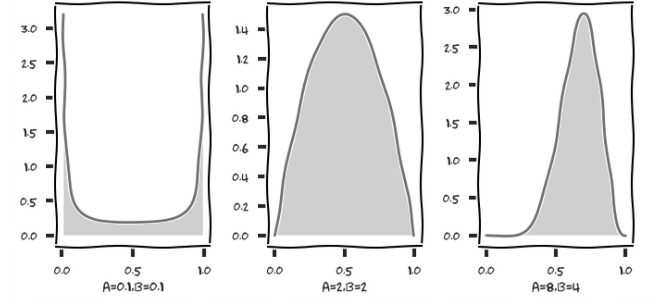
\includegraphics[scale=.6]{img/betaExamples.png}

\definition{Direchlet Distribution}
Let $X\sim\text{Dir}(\pmb{\alpha})$. Then
$$f_X(x):=\dfrac{\Gamma(\alpha_0)}{\Gamma(\alpha_1)\times\dots\times\Gamma(\alpha_N)}\prod_{i=1}^Nx_i^{\alpha_{i-1}}$$

\definition{Exponential Distribution Family}
The \textit{Exponential Distribution Family} is a set of probability distributions which fit the form.
$$\prob(\x|\pmb{\theta})=h(\x)g(\pmb{\theta})e^{\pmb{\theta}^T\textbf{u}(\x)}$$
With conjugate prior
$$\prob(\pmb{\theta}|\pmb{\chi},\nu)=f(\pmb{\chi},\nu)g(\pmb{\chi})^\nu e^{\nu\pmb{\theta}^T\pmb{\chi}}$$

\definition{Multivariate Normal Distribution}
Let $\X\sim\mathcal{N}(\mub,\pmb{\Sigma})$. Then
$$f_\X(\x)=\dfrac{1}{(2\pi)^{N/2}|\pmb{\Sigma}^{1/2}}e^{-\frac{1}{2}(\x-\mub)^T\pmb{\Sigma}^{-1}(\x-\mub)}$$
\nb Also known as \textit{Gaussian Distribution}.

\section{Regression}

\definition{Supervised Learning}
Learning the relationship $f(\cdot)$ between pairs of data $x_i$ and $y_i$ where $y_i=f(x_i)$.\\

\remarkk{Summary of Regression}
\begin{itemize}
	\item[Linear Regression] We are limited to lines
	\item[Basis Functions Regression] We can use non-linear functions, but it is hard to determine how many \& what basis functions should be used. The prior is hard to interpret.
	\item[Kernel Regression] The complexity is defined by the data (Good) but there is no uncertainty in our estimate.
\end{itemize}

\subsection{Linear Regression}

\definition{Linear Regression}
\textit{Linear Regression} is the process of taking a set of data points \& producing a linear relationship between a dependent varaible \& one of more explanatory variables.\\
Let $\x\in\reals^n$ be a set of observed values from $n$ explanatory variables \& $\textbf{a}\in\reals^n+1$ be a set of parameters. Then we predict the value of the dependent variable to be
$$y(\x,\textbf{a})=a_0+\sum\limits_{i=0}^na_{i+1}x_i$$

\remark{Limitation of Linear Regression}
The formula defined in \textbf{Definition 3.1} is a linear function of the coefficients defined by $\textbf{a}$ \textbf{and} the observed values of $\x$ this limits the relationships we can model between elements of $\x$. The model can be extended to avoid this using \textit{Basis Functions}.\\

\definition{Linear Regression - Basis Functions}
We can extend \textit{Linear Regression} to include \textit{Basis Functions} so that relationships between explanatory variables can be modelled.\\
Let $\x\in\reals^n$ be a set of observed values from explanatory variables, $\textbf{a}\in\reals^{m}$ be a set of coefficients (weightings), and $\pmb{\phi}:\reals^n\to\reals^{m-1}$ be a set of basis functions. Then we can predict the dependent variable to be
$$y(\x,\textbf{a})=a_0+\sum_{i=1}^ma_i\phi_{i-1}(\x)$$

\remark{Linear Regression - Basis Function}
To simplfy the equation used in \textbf{Definition 3.2} we can define $\pmb{\phi}:\reals^n\to\reals^m$ with $\phi_0(\x)$. Then
$$y(\x,\textbf{a})=\sum_{i=0}^ma_i\phi_i(\x)=\textbf{a}^T\pmb{\phi}(\x)$$

\proposition{Noise}
We will often introduce the concept of \textit{Noise} into a \textit{Linear Regression} model. Typically we assume noise to be modelled by a zero-mean Normal distribution with precision $\beta$, $\varepsilon\sim\text{Normal}(0,\beta^{-1})$, so
$$t:=y(\x,\textbf{a})=\textbf{a}^T\pmb{\phi}(\x)+\varepsilon$$
From this we can derive a likelihood
$$\prob(t|\x,\textbf{a},\beta)\sim\text{Normal}(t|\mu=y(\x,\textbf{a}),\sigma^2=\beta^{-1})=\text{Normal}(t|\mu=\textbf{a}^T\pmb{\phi}(\x),\sigma^2=\beta^{-1})$$
If we have a series of sets of observations, $\X\in\reals^{m\times n}$, then
$$\prob(\textbf{t}|\X,\textbf{a},\beta)\sim\prod\limits_{i=1}^m\text{Normal}(t_i|\mu=\textbf{a}^T\pmb{\phi}(\x_i),\sigma^2=\beta^{-1})$$
%TODO what is precision v variance in normal distribution

\definition{Maximum Likelihood Estimate}
A \textit{Maximum Likelihood Estimate} is estimating the value of a parameter to be the most likely, according to our \textit{Likelihood Function}.\\

\remark{Finding Maximum Likelihood Estimate}
Suppose we have a defined \textit{Likelihood Function} $\prob(\textbf{t}|\X,\textbf{a},\beta)$ and we want to find \textit{Maximum Likelihood Estimates} for parameters $\textbf{a}$. Then
\begin{enumerate}[label=\roman*)]
	\item Define the \textit{Likelihood Function}, $\prob(\textbf{t}|\X,\textbf{a},\beta)$.
	\item Take the natural log, $\ln\prob(\textbf{t}|\X,\textbf{a},\beta)$.
	\item Take the derivative wrt $\textbf{a}$, $\frac{\partial}{\partial\textbf{a}}\ln\prob(\textbf{t}|\X,\textbf{a},\beta)$.
	\item Set the derivatite to $0$, $\frac{\partial}{\partial\textbf{a}}\ln\prob(\textbf{t}|\X,\textbf{a},\beta)=0$.
	\item Solve to find the stationary point of $\textbf{a}$.
	\item Check this stationary point is a maximum, if it is then it is a \textit{Maximum Likelihood Estimate}
\end{enumerate}

\example{Maximum Likelihood Estimate}
Here I shall find the \textit{Maximum Likelihood Estimate} for $\textbf{a}$
\[\begin{array}{rrcl}
&\prob(\textbf{t}|\X,\textbf{a},\beta)&\sim&\prod\limits_{i=1}^m\text{Normal}(t_i|\textbf{a}^T\pmb{\phi}(\x_i),\beta^{-1})\\
&&=&\prod\limits_{i=1}^m\dfrac{1}{\sqrt{2\pi\beta^{-1}}}e^{-\frac{1}{2}\beta(t_i-\textbf{a}^T\pmb{\phi}(x_i))^2}\\
&&=&\left(\frac{\beta}{2\pi}\right)^{\frac{m}{2}}e^{-\frac{\beta}{2}\sum\limits_{i=1}^m(t_i-\textbf{a}^T\pmb{\phi}(x_i))^2}\\
\implies&\ln\prob(\textbf{t}|\X,\textbf{a},\beta)&=&\frac{m}{2}(\underbrace{\ln(\beta)}_{\text{Noise Precision}}-\underbrace{\ln(2\pi)}_{\text{Constant}})-\underbrace{\frac{\beta}{2}\sum\limits_{i=1}^m(t_i-\textbf{a}^T\pmb{\phi}(x_i))}_{\text{Error}}\\
\implies&\frac{\partial}{\partial\textbf{a}}\ln\prob(\textbf{t}|\X,\textbf{a},\beta)&=&\beta\sum\limits_{i=1}^2(\textbf{t}_i-\textbf{a}^T\pmb{\phi}(\x_i))\pmb{\phi}(x_i)^T\\
\text{Setting}&0&=&\frac{\partial}{\partial\textbf{a}}\ln\prob(\textbf{t}|\X,\textbf{a},\beta)\\
\implies&0&=&\beta\sum\limits_{i=1}^2(\textbf{t}_i-\textbf{a}^T\pmb{\phi}(\x_i))\pmb{\phi}(x_i)^T\\
&&=&\left(\sum\limits_{i=1}^m\textbf{t}_i\pmb{\phi}(\x_i)^T\right)-\textbf{a}^T\left(\sum\limits_{i=1}^m\pmb{\phi}(\x_i)\pmb{\phi}(\x_i)^T\right)\\
\implies&\textbf{a}_{MLE}&=&\left(\pmb{\phi}(\X)^T\pmb{\phi}(\X)\right)^{-1}\pmb{\phi}(\X)^T\textbf{t}
\end{array}\]

\theorem{Variance of Posterior}
Let $\alpha$ be the parameter of the prior, $\beta$ be the parameter for the likelihood and $\X$ be the observed values from the predictor variables.
%TODO not sure of these definitions
\[\begin{array}{rcl}
s_n&=&(I\alpha+\beta \X^T\X)^{-1}\\
&=&\left(I\alpha+\beta\begin{pmatrix}
\sum\limits_{i=1}^n1&\sum\limits_{i=1}^nx_i\\
\sum\limits_{i=1}^nx_i&\sum\limits_{i=1}^nx_i^2
\end{pmatrix}\right)^{-1}\\
&=&\begin{pmatrix}
\beta n+\alpha&\beta\sum\limits_{i=1}^nx_i\\
\beta\sum\limits_{i=1}^nx_i&\alpha+\beta\sum\limits_{i=1}^nx_i^2
\end{pmatrix}^{-1}\\
&=&\dfrac{1}{(\beta n+\alpha)\left(\alpha+\beta\sum\limits_{i=1}^nx_i^2\right)-\left(\beta\sum\limits_{i=1}^nx_i\right)^2}\begin{pmatrix}
\alpha+\beta\sum\limits_{i=1}^nx_i^2&-\beta\sum\limits_{i=1}^nx_i\\
-\beta\sum\limits_{i=1}^nx_i&\beta n+\alpha
\end{pmatrix}\\
&&\text{Assume data is centred so }\sum\limits_{i=1}^nx_i=0\\
&=&\dfrac{1}{(\beta n+\alpha)\left(\alpha+\beta\sum\limits_{i=1}^nx_i^2\right)}\begin{pmatrix}
\alpha+\beta\sum\limits_{i=1}^nx_i^2&0\\
0&\beta n+\alpha
\end{pmatrix}\\
&=&\begin{pmatrix}
\dfrac{1}{\beta n+\alpha}&0\\
0&\dfrac{1}{\alpha+\beta\sum\limits_{i=1}^nx_i^2}
\end{pmatrix}
\end{array}\]

\theoremm{Mean of Posterior}
Let $\alpha$ be the parameter of the prior, $\beta$ be the parameter for the likelihood, $\X$ be the observed values from the predictor variables and $\textbf{t}$ be the observed values for the dependent variable.
\[\begin{array}{rcl}
m_n&=&(\alpha I+\beta \X^T\X)^{-1}\beta \X^T\textbf{t}\\
&=&s_n\beta\X^T\textbf{t}\\
&=&\beta s_n\begin{pmatrix}
1&\dots&1\\
x_1&\dots&x_n
\end{pmatrix}
\begin{pmatrix}
t_1\\
\vdots\\
t_n
\end{pmatrix}\\
&=&\beta s_n\begin{pmatrix}
\sum\limits_{i=1}^nt_i\\
\sum\limits_{i=1}^nt_ix_i
\end{pmatrix}\\
&&\text{Assume data is centred so }\sum\limits_{i=1}^nx_i=0\\
&=&\beta\begin{pmatrix}
\dfrac{1}{\beta n+\alpha}&0\\
0&\dfrac{1}{\alpha+\beta\sum\limits_{i=1}^nx_i^2}
\end{pmatrix}\begin{pmatrix}
\sum\limits_{i=1}^nt_i\\
\sum\limits_{i=1}^nt_ix_i
\end{pmatrix}\\
&=&\begin{pmatrix}
\dfrac{\beta\sum_{i=1}^nt_i}{\beta n+\alpha}\\
\dfrac{\beta\sum_{i=1}^nt_ix_i}{\alpha+\beta\sum_{i=1}^nx_i^2}
\end{pmatrix}
\end{array}\]

\proposition{Prediction}
Suppose we are given as inputs to the model: $\X$ observations from the predictor variables, $\textbf{t}$ observations from the dependent variable; $\alpha$, parameter for the prior; and $\beta$, parameter for the likelihood.\\
If we now want to predict the value $\hat{t}$ at position $\hat{\x}$ we want to solve
$$\prob(\hat{t}|\hat{\x},\textbf{t},\X,\alpha,\beta)=\int\prob(\hat{t}|\hat{\x},\textbf{a},\beta)\prob(\textbf{a}|\textbf{t}|\X,\alpha,\beta)d\textbf{a}$$
where $\textbf{a}$ is the coefficient for weighting each parameter.

\subsection{Dual Linear Regression}

\definition{Kernel}
A \textit{Kernel} is a function that defines an inner-produce in some space.\\
Let $\x$ be a vector in the orignal space \& $\phi(\cdot)$ map from the original space to the kernel space. Then the \textit{Kernel Function} is defined as
$$k(\x_i,\x_j):=\phi(\x_i)^T\phi(\x_j)$$

\remark{Usefulness of Kernels}
It is generally easier to define the inner-product of a space than to define a space \& kernels allow us to never have to realise a space. This allows us to work with infinite dimensional spaces.\\
\nb The space defined by the \textit{Kernel} is called the \textit{Induced Space}.\\

\definition{Kernel Regression}
\textit{Kernel Regression} is the act of performing a linear regression in an \textit{Induced Space}.\\
Let $\X$ \& $\textbf{t}$ be  training data, $\lambda$ be a parameter for noise, $\hat{\x}$ be an unseen data point which we wish to predicit a value $\hat{y}$ for. Then
$$\hat{y}(\hat{\x})=k(\hat{\x},\x)(k(\X,\X)+\lambda I)^{-1}\textbf{t}$$

\remark{Usefulness of Kernel Regression}
Note that the problem is linear in the \textit{Induced Space} but not in the original space, thus allowing us to learn non-linear functions using lines.\\


\remark{Changing Basis}
Some data is clearly non-linear \& it may be helpful to transform it into another basis where linear regression is possible.\\
\eg If the data appearas to fit a circle in a cartesian basis, it can be translated into polar co-ordinates which should be linear.\\
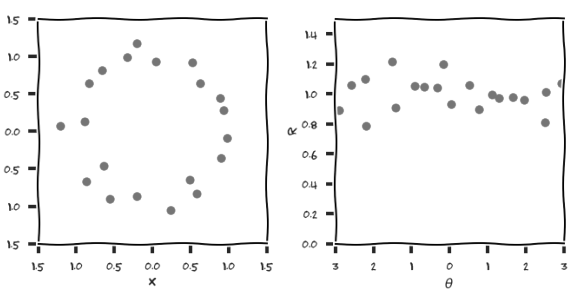
\includegraphics[scale=.4]{img/changeBasis.png}

\proposition{Changing Basis}
Let $\textbf{a}$ be weightings for observed parameters and $\x$ be a set of observed parameters.\\
Suppose we want to change the basis of $\x$, if we have a function $\phi:\mathcal{X}\to\mathcal{Z}$ which can do this then we predict $y$ as
$$t=\textbf{a}^T\phi(\x)=\textbf{a}^T\textbf{z}$$

\definition{Dual Linear Regression}
Standard \textit{Linear Regression} is defined as a linear combination of columns. \textit{Dual Linear Regression} is a linear combination of the inner product of a new data point with each of the training data, this allows it to consider combinations of data points.\\

\remark{Intution of Dual Regression}
\textit{Dual Regression} can be considered as describing an unseen data points as a combination of seen ones. \ie Has the shape of a rhino, fur of a tiger, ...\\

\proposition{Dual Linear Regression Steps}
To perform a \textit{Dual Linear Regression} perform the following
\begin{enumerate}[label=\roman*)]
	\item Formulate Posterior, $\prob(\theta|\X)$;
	\item Find stationary point of posterior;
	\item Re-write the coefficients $\textbf{a}$ in terms of the data;
	\item Perform Kernel regression.
\end{enumerate}
%TODO formulae & better explanation of process

\remark{Useful Kernels}
Not all functions can be used as \textit{Kernels}. Some that can, and can be useful,
\begin{enumerate}[label=\roman*)]
	\item Kernelised Euclidean Distance $\|\phi(\x_i)-\phi(\x_j)\|^2=k(\x_i,\x_i)-2k(\x_i,\x_j)+k(\x_j,\x_j)$
	\item Exponented Quadratic $k(\x_i,\x_j)=\sigma^2 e^{-\frac{1}{2\ell^2}(\x_i-\x_j)^T(\x_i-\x_j)}$.
\end{enumerate}

\remarkk{Limitations of Linear/Dual Regression}
\begin{enumerate}[label=\roman*)]
	\item No uncertainty in our observed outputs;
	\item No uncertainity in our mapping;
	\item We have to make assumptions over the space of functions
\end{enumerate}

\subsection{Gaussian Processes}

\remark{Motivation}
Here we want to introduce uncertainty into our observed outputs \& mappings. This means that instead of outputting a discrete value we return a probability distribution. Now we can consider a few more features for our observations, such as how much does observing a value at $\x_0$ tell us about an observation at $\x_1$.\\
\nb In the image before we have an observation for $x=-2$ and three marginals for $x=-2,3,6$ which our observation has a decreasing affec on, as distance increases.\\
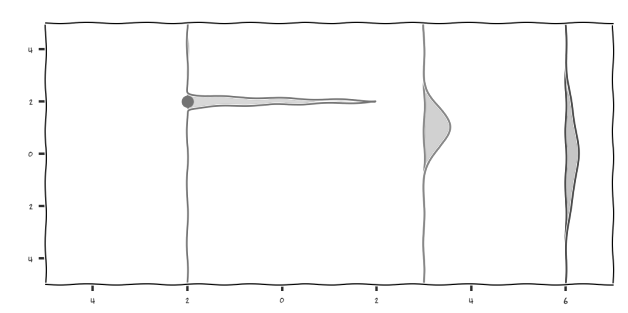
\includegraphics[scale=1]{img/decay.png}

\definition{Gaussian Process}
A \textit{Gaussina Process} is a generalisation of random variables into an infinite number of \textit{Gaussian Distributions}. The specific process is defined by a mean function $\mu(\cdot)$ and a co-variance function function $k(\cdot)$.
$$\prob(f_1,f_2,\dots|\x,\pmb{\theta})\sim\mathcal{GP}\left(\mu(\x),k(\x,\x)\right)=\text{Normal}\left(\begin{pmatrix}
\mu(x_1)\\\mu(x_2)\\\vdots
\end{pmatrix},\begin{pmatrix}
k(x_1,x_1)&k(x_1,x_2)&\dots\\
k(x_2,x_1)&k(x_2,x_2)&\dots\\
\vdots&\vdots&\ddots
\end{pmatrix}\right)$$
\nb \textit{Gaussian Processes} is non-parameteric.\\

\remark{Covariance Function}
The \textit{Covaraince Function} of a \textit{Gaussian Process} defines how much an observation at $\x_0$ affects our prediction for $\x_1$. The greater the covariance values (Not on the main diagonal) the more an observation tells us. We can define the \textit{Covariance Functions} to vary with distance \& other factors.
$$\text{Very little effect}=\begin{pmatrix}
1&.1\\
.1&1
\end{pmatrix}.\quad\text{A lot of effect}=\begin{pmatrix}
1&.9\\
.9&1
\end{pmatrix}$$

\remark{Sampling from a Gaussian Process}
When we take a sample from a \textit{Gaussian Process} we are given a function which fits the distributions defined the \textit{Gaussian Process}.\\

\example{Sampling from a Gaussian Process}
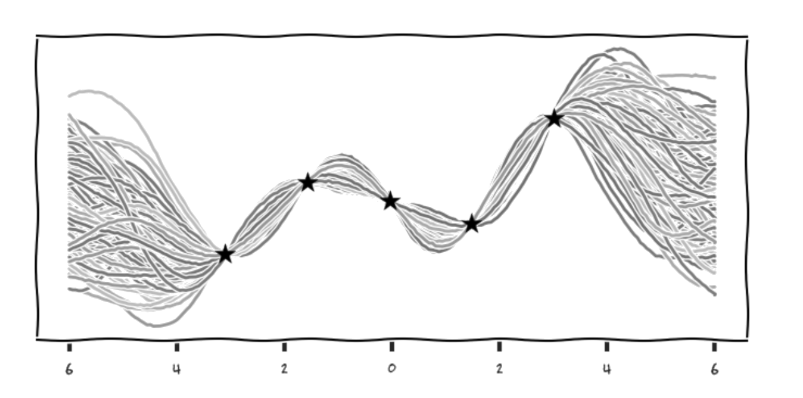
\includegraphics[scale=.7]{img/samplingGaussianProccess.png}

\proposition{Gaussian Process - Posterior, No Noise}
Let $\textbf{f},\X$ be training data, $f^*,\x^*$ be training data and $k$ be the co-variance function. We have %TODO
\[\begin{array}{rcl}\begin{pmatrix}
\textbf{f}\\
f^*
\end{pmatrix}&\sim&\text{Normal}\left(\begin{pmatrix}
\textbf{0}\\
0
\end{pmatrix},\begin{pmatrix}
k(\X,\X)&k(\X,\x^*)\\
k(\x^*,\X)&k(\x^*,\x^*)
\end{pmatrix}\right)\\
\prob(f^*|\x^*,\X,\textbf{f})&\sim&\text{Normal}\bigg(k(\x^*,\X)^Tk(\x^*,\X)^{-1}\textbf{f},\ k(\x^*,\x^*)-k(\x^*,\X)^Tk(\X,\X)^{-1}k(\X,\x^*)\bigg)
\end{array}\]

\proposition{Gaussian Process - Posterior, Noise}
Let $\textbf{f},\X$ be training data, $f^*,\x^*$ be training data and $k$ be the co-variance function.\\ Define $\textbf{y}_i=f_i+\varepsilon$ where $\varepsilon\sim\text{Normal}(0,\sigma^2I)$ We have %TODO
\[\begin{array}{rcl}\begin{pmatrix}
\textbf{y}\\
f^*
\end{pmatrix}&\sim&\text{Normal}\left(\begin{pmatrix}
\textbf{0}\\
0
\end{pmatrix},\begin{pmatrix}
k(\X,\X)+\sigma^2I&k(\X,\x^*)\\
k(\x^*,\X)&k(\x^*,\x^*)
\end{pmatrix}\right)\\
\prob(f^*|\x^*,\x,\textbf{y},\sigma^2)&\sim&\text{Normal}\bigg(k(\x^*,\x)^T(k(\x,\x)+\sigma^2I)^{-1}\textbf{y},\ k(\x^*,\x^*)-k(\x^*,\x)^T(k(\x,\x)+\sigma^2I)^{-1}k(\x,\x^*)\bigg)
\end{array}\]

\example{Noisy Gaussian Process}
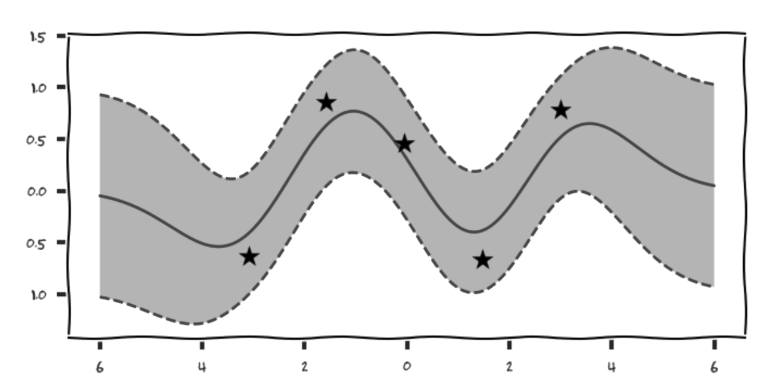
\includegraphics[scale=.7]{img/noisyGaussianProcess.png}

\section{Unsupervised Learning}
%TODO go through NotesLecturer & slides

\definition{Unsupervised Learning}
In \textit{Unsupervised Learning} we are given only the ouput data \& are tasked with deriving the underlying properties of each event.\\
\ie Given $y=f(x)$ recover both $f(\cdot)$ \& $x$.

\section{Bayesian Optimisation}

\remark{Importance of Uncertainty}
Note that we can have $\hat{x}=argmax_xp(x)=\text{argmax}_xq(x)$ but $p(\hat{x})\neq q(\hat{x})$. Due to this we need to introduce uncertainty about the value of $x$ so that we can weight out outcomes accordingly.\\
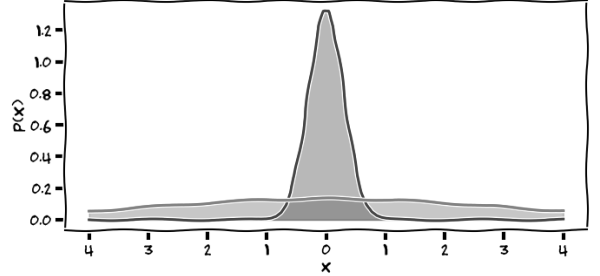
\includegraphics[scale=.4]{img/uncertainty.png}

\definition{Optimisation}
\textit{Optimisation} is the process of finding the best outcome for a problem.\\

\remark{Optimisation}
Classically \textit{Optimisation} is seen as $\hat{x}=\argmin_xf(x)$ however we typically have an objective function that we do not know explicitly, but are able to test. Since testing in real life situations (\eg Medical Trials) are expensive we want to minimise the number required to achieve a good level of certainty.\\

\definition{Global Optimisation}
\textit{Global Optimisation} is the set of techniques for finding $x_M=\argmin_{x\in\mathcal{X}}f(x)$ where $\mathcal{X}$ is a bounded domain (reducing the amount of testing required) and $f$ is not known explicitly. It is possible that evaluations of $f$ are noisy.\\

\propositionn{Bayesian Optimisation}
\begin{enumerate}[label=\roman*)]
	\item Choose a prior over the space of possible objective functions, $f$.
	\item Combine the prior \& likelihood to get a posterior over the space.
	\item Use the posterior to choose a set of evaluations according to a \underline{strategy}ive
	.
	\item Add new data, update posterior \& re-evaluate.
	\item Repeat until budget is gone
\end{enumerate}

\proposition{Na\"ive Strategies for Global Optimisation}
Below are some na\"ive \textit{Global Optimisation} stategies
\begin{enumerate}[label=\roman*)]
	\item Implicity knowledge, ask a SME;
	\item Grid Search, test the domain at regular intervals; and,
	\item Random Sampling.
\end{enumerate}

\remark{Exploration v Exploitation}
When considering strategies for \textit{Bayesian Optimisation} we need to consider how we approach \textit{Exploration} (Testing new areas) \& \textit{Explotation} (Investigating areas which seem good). A \textit{Acquisition Function} can be defined which returns the expected gain in information if a sample was to be taken at $x$.\\

\definition{Expected Improvement}
\textit{Expected Improvement} is an \textit{Acquistion Function}.\\
Let $\x$ be a point in the domain, $\theta$ be parameters of the distribution and $X$ be data we already know. Then
$$EI(\x;\theta,X):=\int\max(0,y_{best}-y)\prob(y|\x,\theta,X)dy$$
We should then sample at $\x$ where $EI(\x)\geq EI(\x')\ \forall\ x'\in\mathcal{X}$ since this point offers the greatest information gain.\\
\nb $y_{best}$ is the best value for $y$ we have found so far. \ie The value we are trying to improve.\\
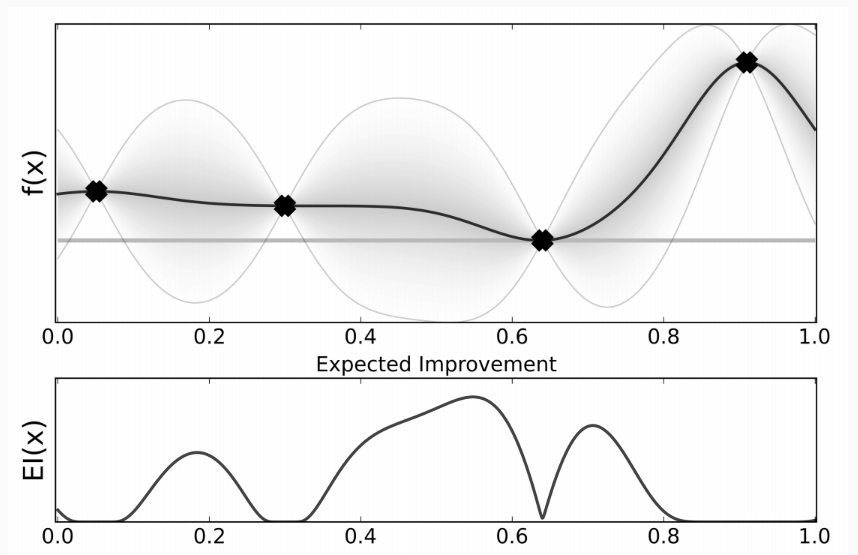
\includegraphics[scale=.4]{img/expectedImprovement.png}

\definition{Thomson Sampling}
\textit{Thomson Sampling} is an \textit{Acquistion Function}.\\
Let $\x$ be a point in the domain, $\theta$ be parameters of the distribution and $X$ be data we already know. Then
$$T(\x;\theta,X):=\prob(y|\x,\x,\theta,X)$$
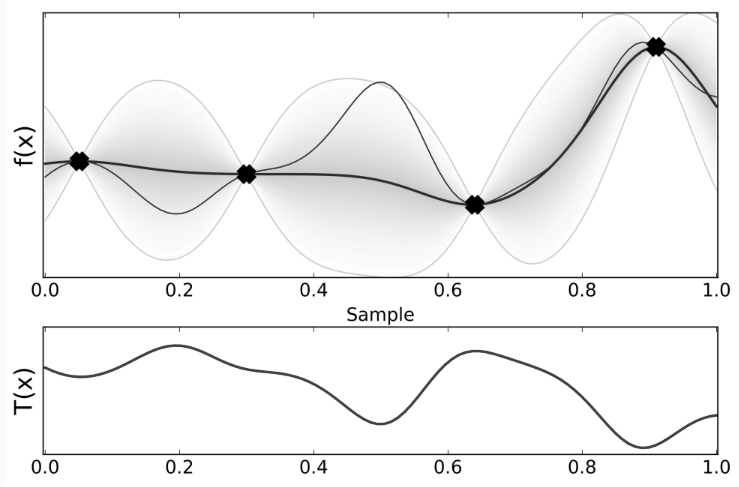
\includegraphics[scale=.4]{img/thomsonSampling.png}

\newpage
\setcounter{section}{-1}
\section{Appendix}

\subsection{Definitions}

\definition{Memory-Based Methods}
\textit{Memory-Based Methods} for classification store the entire training set in order to make predictions for future data points. \eg Nearest-Neighbours.\\
\nb These generally require a distance measure to be defined.\\

\subsection{Proofs}
\proof{Deriving Gaussian Marginal Distribution}
\textit{NOTE - This is dense as fuck \& uses quite a bit of bullshit}.\\
\\Let $\X\sim\mathcal{N}\left(\begin{pmatrix}
\mub_1\\\mub_2
\end{pmatrix},\begin{pmatrix}
\Lambda_{11}&\Lambda_{12}\\
\Lambda_{21}&\Lambda_{22}
\end{pmatrix}^{-1}\right)$.\\
$\mub_1,\mub_2$ can be considered as two parts of the mean vector $\mub$.\\
Let $\x$ be a realisation of $\X$ where $\x:=(\x_1,\x_2)$ with $\x_1\ \&\ \x_2$ representing the same partition as $\mub_1\ \&\ \mub_2$ respecitvely.\\
Define $D:=\mathrm{dim}(\x),\ D_1:=\mathrm{dim}(\x_1)\ \&\ D_2:=\mathrm{dim}(\x_2)$.\\
\\Here we want to get from $\prob(\x_1,\x_2)$ to $\prob(\x_1)$.\\
Consider the exponent of the joint distribution
$$E=-\frac{1}{2}(\x_1-\mub_1)^T\Lambda_11(\x_1-\mub_1)-\frac{1}{2}(\x_1-\mub_1)^T\Lambda_{12}(\x_2-\mub_2)-\frac{1}{2}(\x_2-\mub_2)^T\Lambda_{21}(\x_1-\mub_1)-\frac{1}{2}(\x_2-\mub_2)^T\Lambda_{22}(\x_2-\mub_2)$$
To produce the marginal for $x_1$ we want to isolate the terms involving $x_2$ so they are easy to remove.
\[\begin{array}{rcl}
E&=&-\frac{1}{2}\bigg[\left(\x_2^T\Lambda_{22}\x_2-2\x_2^T\Lambda_22(\mub_2-\Lambda_{22}^{-1}\Lambda_{21}(\x_1-\mub_1))\right)\\
&-&2\x_1^T\Lambda_{12}\mub_2+2\mub_1^T\Lambda_{12}\mub_2+\mub_2^T\Lambda_{22}\mub_2+\x_1^T\Lambda_{11}\x_1\\
&-&2\x_1^T\Lambda_11\mub_1+\mub_1^T\Lambda_{11}\mub_1\bigg]\\
&=&\underbrace{-\frac{1}{2}\left(\x_2-(\mub_2-\Lambda_{22}^{-1}\Lambda_{21}(\x_1-\mub_1))\right)^T\Lambda_{22}\left(\x_2-(\mub_2-\Lambda_{22}^{-1}\Lambda_{21}(\x_1-\mub_1))\right)}_{E_1}\\
&+&\underbrace{\frac{1}{2}\left(\x_1^T\Lambda_{12}\Lambda_{22}^{-1}\Lambda_{21}\x_1-2\x_1^T\Lambda_{12}\Lambda_{22}^{-1}\Lambda_{21}\mub_1+\mub_1^T\Lambda_{12}\Lambda_{22}^{-1}\Lambda_{21}\mub_1\right)}_{A}\\
&-&\underbrace{\frac{1}{2}\left(\x_1^T\Lambda_11\x_1-2\x_1^T\Lambda_{11}\mub_1+\mub_{1}\Lambda_{11}\mub_1\right)}_{B}
\end{array}\]
Note that $A$ \& $B$ do not contain any $x_2$ terms.\\
Since the co-variance matrix is symmetric we have $\Lambda_{12}=\Lambda_{21}^T$ we have
$$\x_1^T\Lambda_{12}\mub_2=\x_1^T\Lambda_{21}^T\mub_2=(\Lambda_{21}\x_1)^T\mub_2=\mub_2^T\Lambda_{21}\x_1$$
We shall not rewrite $A$ \& $B$ as quadratic expressions
\[\begin{array}{rrcl}
&A&=&\dfrac{1}{2}\left(\x_1^T\Lambda_{12}\Lambda_{22}^{-1}\Lambda_{21}\x_1-2\x_1^T\Lambda_{12}\Lambda_{22}^{-1}\Lambda_{21}\mub_1+\mub_1^T\Lambda_{12}\Lambda_{22}^{-1}\Lambda_{21}\mub_1\right)\\
&&=&\dfrac{1}{2}(\x_1-\mub_1)^T(\Lambda_{12}\Lambda_{22}^{-1}\Lambda_{21})(\x_1-\mub_1)\\
&B&=&\dfrac{1}{2}\left(\x_1^T\Lambda_{11}\x_1-2\x_1^T\Lambda_{11}\mub_1+\mub_{1}\Lambda_{11}\mub_1\right)\\
&&=&\dfrac{1}{2}(\x_1-\mub_1)^T\Lambda_{11}(\x_1-\mub_1)\\
\implies&A-B&=&\frac{1}{2}(\x_1-\mub_1)^T(\Lambda_{12}\Lambda_{22}^{-1}\Lambda_{21}-\Lambda_{11})(\x_1-\mub_1)\\
&\mathrm{Let\ }E_2&:=&A-B
\end{array}\]
Now the exponent has been orgainised we can consider the whole gaussian expression.
\[\begin{array}{rcll}
\prob(\x_1,\x_2)&=&\dfrac{e^{E_1}e^{E_2}}{(2\pi)^{\frac{D}{2}}|\Sigma|^{\frac{1}{2}}}\\
\prob(\x_1)&=&{\displaystyle\int\prob(\x_1,\x_2)d\x_2}\\
&=&{\displaystyle\int\dfrac{e^{E_1}e^{E_2}}{(2\pi)^{\frac{D}{2}}|\Sigma|^{\frac{1}{2}}}d\x_2}\\
&=&{\dfrac{e^{E_2}}{(2\pi)^{\frac{D}{2}}|\Sigma|^{\frac{1}{2}}}\displaystyle\int e^{E_1}d\x_2}&\text{Since $E_2$ is independent of $\x_2$}
\end{array}\]
Now we consider $\int e^{E_1}d\x_2$.\\
Since we know a gaussian must intergrate to 1 over the whole domain we deduce that
\[\begin{array}{rrcl}
&{\displaystyle\int\dfrac{1}{(2\pi)^{\frac{D_2}{2}}|\Lambda_{22}^{-1}|^{\frac{1}{2}}}e^{E_1}d_{\x_2}}&=&1\\\
\implies&\int e^{E_1}d\x_2&=&(2\pi)^{\frac{D_2}{2}}|\Lambda_{22}^{-1}|^{\frac{1}{2}}
\end{array}\]
\nb $\Lambda_{22}^{-1}$ is the variance of $\x_2$.\\
Using the result of this intergal we have
\[\begin{array}{rcl}
\prob(\x_1)&=&(2\pi)^{\frac{D_2}{2}}|\Lambda_{22}^{-1}|^{\frac{1}{2}}\dfrac{1}{(2\pi)^{\frac{D}{2}}|\Sigma|^{\frac{1}{2}}}e^{E_2}\\
&=&\dfrac{e^{E_2}}{(2\pi)^{\frac{D-D_2}{2}}|\Lambda_{22}^{-1}|^{-\frac{1}{2}}|\Sigma|^{\frac{1}{2}}}
\end{array}\]
The Schur complement of $\Lambda_{22}$ is $\Lambda^{-1}_{22}=\Sigma_{22}-\Sigma_{21}\Sigma_{11}^{-1}\Sigma_{12}$.\\
Thus \[\begin{array}{rcl}
|\Lambda_{22}^{-1}|^{-\frac{1}{2}}|\Sigma|^{\frac{1}{2}}&=&|\Sigma_{22}-\Sigma_{21}\Sigma_{11}^{-1}\Sigma_{12}|^{-\frac{1}{2}}|\Sigma_{11}|^{\frac{1}{2}}|\Sigma_{22}-\Sigma_{21}\Sigma_{11}^{-1}\Sigma_{12}|^{\frac{1}{2}}\\
&=&|\Sigma_{11}|^{\frac{1}{2}}
\end{array}\]
Now we have a full expression
\[\begin{array}{rcl}
\prob(\x_1)&=&\dfrac{e^{E_2}}{(2\pi)^{\frac{D-D_2}{2}}|\Lambda_{22}^{-1}|^{-\frac{1}{2}}|\Sigma|^{\frac{1}{2}}}\\
&=&\dfrac{1}{(2\pi)^{\frac{D_1}{2}}|\Sigma_{11}|^{\frac{1}{2}}}e^{-\frac{1}{2}(\x_1-\mub_1)^T\Sigma_{11}^{-1}(\x_1-\mub_1)}
\end{array}\]
$\hfill{\blacksquare}$

\proof{Deriving Gaussian Conditional Distribution}
\\Let $\X\sim\mathcal{N}\left(\begin{pmatrix}
\mub_1\\\mub_2
\end{pmatrix},\begin{pmatrix}
\Sigma_{11}&\Sigma_{12}\\
\Sigma_{21}&\Sigma_{22}
\end{pmatrix}\right)$.\\
$\mub_1,\mub_2$ can be considered as two parts of the mean vector $\mub$.\\
Let $\x$ be a realisation of $\X$ where $\x:=(\x_1,\x_2)$ with $\x_1\ \&\ \x_2$ representing the same partition as $\mub_1\ \&\ \mub_2$ respecitvely.\\
Define $D:=\mathrm{dim}(\x)$.\\
\\We want to find the distribution of $\prob(\x_1|\x_2)$.\\
From the product rule we know that $\prob(\x_1,\x_2)=\prob(\x_1|\x_2)\prob(\x_2)$ and we already know the joint \& marginal distributions for a gaussian.\\
We have that
$$
\prob(\x_1,\x_2)\propto e^{-\frac{1}{2}\begin{pmatrix}
\x_1-\mub_1\\\x_2-\mub_2
\end{pmatrix}^T\begin{pmatrix}
\Sigma_{11}&\Sigma_{12}\\
\Sigma_{21}&\Sigma_{22}
\end{pmatrix}^{-1}\begin{pmatrix}
\x_1-\mub_1\\\x_2-\mub_2
\end{pmatrix}}$$
We now want to factor the marginal distribution out of this expression.
$$
\prob(\x_2)\propto e^{-\frac{1}{2}(\x_2-\mub_2)^T\Sigma_{22}^{-1}(\x_2-\mub_2)}
$$
Lets look at the exponent of the joint distribution.\\
\nb About to use a lot of Schur Complements
\[\begin{array}{rl}
E&=-\dfrac{1}{2}\begin{pmatrix}
\x_1-\mub_1\\\x_2-\mub_2
\end{pmatrix}^T\begin{pmatrix}
\Sigma_{11}&\Sigma_{12}\\
\Sigma_{21}&\Sigma_{22}
\end{pmatrix}^{-1}\begin{pmatrix}
\x_1-\mub_1\\\x_2-\mub_2
\end{pmatrix}\\
&=-\dfrac{1}{2}\begin{pmatrix}
\x_1-\mub_1\\
\x_2-\mub_2
\end{pmatrix}^T
\begin{pmatrix}
I&0\\
\Sigma_{22}^{-1}\Sigma_{21}&I
\end{pmatrix}^T
\begin{pmatrix}
(\Sigma/\Sigma_{22})^{-1}&0\\
0&\Sigma_{22}^{-1}
\end{pmatrix}
\begin{pmatrix}
I&-\Sigma_{12}\Sigma_{22}^{-1}\\
0&I
\end{pmatrix}
\begin{pmatrix}
\x_1-\mub_1\\
\x_2-\mub_2
\end{pmatrix}\\
&=-\dfrac{1}{2}\begin{pmatrix}
\x_1-\mub_1\\
\x_2-\mub_2
\end{pmatrix}^T
\begin{pmatrix}
(\Sigma/\Sigma_{22})^{-1}&-(\Sigma/\Sigma_{22})^{-1}\Sigma_{12}\Sigma_{22}^{-1}\\
-\Sigma_{21}\Sigma_{22}^{-1}(\Sigma/\Sigma_{22})^{-1}&\Sigma_{22}^{-1}
\end{pmatrix}^{-1}
\begin{pmatrix}
\x_1-\mub_1\\
\x_2-\mub_2
\end{pmatrix}\\
&=-\dfrac{1}{2}\bigg[\x_1-(\mub_1+\Sigma_{21}\Sigma_{22}^{-1}(\x_2-\mub_2))\bigg]^T(\Sigma/\Sigma_{22})^{-1}\bigg[\x_1-(\mub_1+\Sigma_{21}\Sigma_{22}^{-1}(\x_2-\mub_2))\bigg]\\
&\underbrace{-\dfrac{1}{2}(\x_2-\mub_2)^T\Sigma_{22}^{-1}(\x_2-\mub_2)}_{E_2}
\end{array}\]
Note that $E_2$ is exactly the exponent for the marginal distribution of $\x_2$ and thus what we want to factory out in order to get to the conditional distribution.
$$\prob(\x_1|\x_2)\propto e^{-\dfrac{1}{2}\big[\x_1-\underbrace{(\mub_1+\Sigma_{21}\Sigma_{22}^{-1}(\x_2-\mub_2))}_{\text{mean}}\big]^T(\underbrace{\Sigma/\Sigma_{22}}_{\text{covariance}})^{-1}\big[\x_1-(\mub_1+\Sigma_{21}\Sigma_{22}^{-1}(\x_2-\mub_2))\big]}$$
$\hfill{\square}$

\subsection{Remarks}

\remark{Worlds}
We can consider 3 different when answering an ml question.
\begin{enumerate}[label=\roman*)]
	\item Deterministic, $x=4$;
	\item Point Estimate, $\text{argmax}_xp(x)=4$;
	\item Stochastic, $p(x)\sim\text{Normal}(4,10^2)$.
\end{enumerate}

\end{document}
